\documentclass[12pt,a4paper]{article}
\usepackage{polski}
\usepackage[utf8]{inputenc}
\usepackage[T1]{fontenc}
\usepackage[margin = 0.5in, top = 1in]{geometry}
\usepackage{fancyhdr}
\usepackage{physics}
\usepackage{amssymb}
\usepackage{graphicx}
\usepackage{hyperref}
\usepackage{float}
\usepackage{subfig}
\usepackage{verbatim}
\usepackage{svg}
\usepackage{textgreek}
\usepackage{tikz}
\usetikzlibrary{bayesnet}
\usepackage[doublespacing]{setspace}
\usepackage[toc,page]{appendix}
\restylefloat{table}
\pagestyle{fancy}
\fancyhf{}
\newcommand{\Ti}{Statistical Data Analysis 2}
\newcommand{\Author}{Mateusz Kapusta}
\newcommand{\dane}{\mathcal{D}}
\newcommand{\Title}{Statistical Data Analysis 2}
\title{\huge \bf \Title\\}
\author{Mateusz Kapusta}
\DeclareRobustCommand{\bbone}{\text{\usefont{U}{bbold}{m}{n}1}}
\DeclareMathOperator{\EX}{\mathbb{E}}% expected value
\rhead{\it \Ti}
\lhead{\Author}
\begin{document}
\maketitle
\section{Start}
Grading rules
\begin{itemize}
    \item 50\% exam (test as usuall)
    \item 15\% and 15\% for two labolatory projects
    \item 15\% midterm test
    \item 5\% lab activity
\end{itemize}
Pass with 50\% as usual.

\section{Lets gooooo}
First some formulas. We denote joint probability of  $mathcal{D}$ and $Y$ $P(X,Y)$. As we know:
\begin{equation}
    P(\mathcal{D})=\sum_{Y}P(X,Y)
\end{equation}
. Then we have conditional probability 
\begin{equation}
    P(\mathcal{D}|Y)=\frac{P(X,Y)}{P(Y)}
\end{equation}
Theeeen
\begin{equation}\label{bayes}
    P(\mathcal{D}|Y)=P(Y|X)\frac{P(X)}{P(Y)}
\end{equation}
aka Bayes theorem.
\subsection{Statistical inference}
Let try to reanalyse coin toss experiment. Let's assume that we have $\theta$ as our propability of heads. When we act in frequentist approach we want to estimate parameter
$\theta$ using methodes as MLE. What we need to claryify we belive there is God's rule that there exist one and only $\theta$ value. In Bayesian framework we do not think aobut tru parameter but 
rather conditional probability $P(\theta|mathcal{D})$ ($X$ is observed data). Lets introduce
\begin{equation}
    L(\theta)=P(mathcal{D}|\theta)
\end{equation}
As we know
\begin{equation}
    P(\mathcal{D}|\theta)=\theta^k(1-\theta)^{N-k}
\end{equation}
When we have $N$ tosses and $k$ sucesses. We can of course use ML estimator and will in the limit converge.
We take logliklihood
\begin{equation}
    l(\theta)=k\log\theta+(N-k)\log{(1-\theta)}
\end{equation}
In ML approach we know that $\hat{\theta}=\frac{k}{N}$ but we want more then point estimator! In frequentist approach we know we can use something like repeat data generating process 
but we can clearly see that this approach isn't going to be very usefull. There is better way, we can use propability to obtain $k$ times sucess.
\begin{equation}
    P(\hat{\theta})=\theta^{\hat{\theta}N}(1-\theta)^{N(1-\hat{\theta})}{N \choose \hat{\theta}N }
\end{equation}
So we know that we can in fact obtain prob denisty for $\hat{\theta}$. It is possible to conduct analysis of propability when we do something like bootstrap. In 
bayesian statistics we think about prior. It is purly our belif about the propability of parameter. Lets decompose \ref{bayes}.
\begin{itemize}
    \item $P(\theta|\mathcal{D})$ - posterior
    \item $P(\mathcal{D}|\theta)$ - likelihood
    \item $P(\theta)$ - prior
    \item $P(\mathcal{D})$ - constant
\end{itemize}
Sometimes life is hard (and we need to use MCMC), sometimes is easy (if we choose easy prior known and conjugate prior) so choose wisely. One of the conjugate priors is 
beta distribution (for binomial likelihood).
\begin{equation}
    \mathcal{B}(\theta|\alpha,\beta)=\frac{\Gamma(\alpha+\beta)}{\Gamma(\alpha)+\Gamma(\beta)}\theta^{\alpha-1}(1-\theta)^{\beta-1}
\end{equation}
This distribution is defined on $[0,1]$ and if $\beta=1$ and $\alpha=1$ we get uniform prior (in other cases it looks very diffrent so we can choose something that suits us).
We also have mean of the distribution at $\mu=\frac{\alpha}{\beta+\alpha}$ so making $\alpha>>\beta$ makes distribution shifted to the right.
Lets rewind
\begin{equation}
    P(\mathcal{D}|\theta)={N\choose k}\theta^k(1-\theta)^{N-k}
\end{equation}
When we use Beta distribution as prior we get posterior
\begin{equation}
    P(\theta|\mathcal{D})=\mathcal{B}(\theta|k+\alpha,N-k+\beta)
\end{equation}
so we know that posterior is very nice.
Now lets introduce some new point estimators
\begin{itemize}
    \item MAP (Maximum aposteriori estimate) $\theta_{MAP}=argmax_{\theta}P(\theta|\mathcal{D})$
    \item ML (Maximum likelihood estimate) $\theta_{ML}=argmax_{\theta}P(\mathcal{D}|\theta)$
\end{itemize}
In the limit of the number of samples both estimators converge to the same value due to the fact that prior is dominativ. With know data prior dominates and things differ.
\section{Bayesian networks}
Bayesian network consist of 
\begin{itemize}
    \item directed acyclic graph (DAG) $G=(V,E)$
    \item local propability distribution, one for each vertex
\end{itemize}
Propabilit distribution for joint values $X=(X_1,\ldots,X_l)$ is
\begin{equation}
    P(X)=\Pi_{i} P(X_i|pa(X_i))
\end{equation}
so we just multiply over conditional propabilities between node and it's parrent.
We can consider something like linear gaussian model so we have 
\begin{equation}
    P(X_n|pa(X_{n}))=Norm(b_n+\omega_{n}^{t}X_{pa(n)},va_n)
\end{equation}
so each vertex is charaterized by two values, mean and covariance matrix.
\subsection{Markov Blancket}
Markov blancket is subset of Bayesian is set of parents, coparents and children for given vertex. It is usefull as it contains all informations to calculate conditional propability of
value of given vertex. We can say, that $P(V| all)=P(V|MB(V))$. Simplifing things we can say that
\begin{equation}
    P(V|all)=P(V|MB(V))=\frac{\sum P(V|parents)+P(children|V,coparents)}{Normalization}
\end{equation}
So it is important when we are sampling using MCMC. 
\subsection{Conditional independence}
We say that $A$ and $B$ are conditional independent given $C$ and wreite $A \perp B |C$. If $A$ and $B$ are children of $C$ then we have conditional independence, the same
when there is connection between $A$ and $B$ through $C$ but not when $C$ is child of $A$ and $B$. In fact, when $A$ and $B$ meet head to head we have independence but not conditional independence.
Now let write some more definitions
\begin{itemize}
    \item let $A$ and $B$ amd $z$ is set of other nodes
    \item If the arrows between our points meet head to head and head to tail path is blocked.
    \item If the arrows meet at node $C$ heat to head and nether the node nor it's desendence belong to $z$ (no "explaining" away)
\end{itemize}
\section{Time to learn}
We can decompose learing process to parameter learning (modeling parameters of graph) and structure learning (determining structure of network).
We can know structure of graph, know all data or any combination.
\subsection{Known graph, known data}
Well, we can just use MAP estimation and we are fine. We treat given parameter as random varible (hidden), assume we have some hyperparameters, we take some prior and then just use MAP.
In discrete case we use something like binomial distribution. In case of many posisble outcomes we can use multinomial distribution (with conjugate prior in form of dirichlet distrubution).
\subsection{Known data, unknown graph}
Well, just want to know the model, we can write
\begin{equation}
    P(G|D)\propto P(D|G)P(G)=\int P(D|G,\theta)P(\theta|G)P(G)\dd\theta
\end{equation}
Its bad but we can sample. One important thing - Bayes factor $\frac{p(\mathcal{D}|M_i)}{P(\mathcal{D}|M_j)}$. It is used to decide which model is better.
\subsection{Markov chains as examples of bayesian networks}
Lets think of the chain that is composed of $N$ parts $X_i$. Because we have chain $X_i$ is dependent only on $X_{i-1}$. When we have Markov property 
\begin{equation}
    P(X_i|X_{i-1})=P(X_2|X_1)
\end{equation}.
As always when dealing with markov chains we have also classical transition matrix $T$. Example: CpG islands. We considere DNA sequence. Sometimes
CG pars will be more often then others what is caled CpG island. When we have supervised learing and somebody gave us some data labeld as cpg or not cpg ilands we can imagine, that
we have two models for two cases labeld $T^+$, $T^-$. We then can use something like log-odds 
\begin{equation}
    S(X)=\log{\frac{P(X|T^+)}{P(X|T^-)}}
\end{equation}. We can set a threshold for clasification and we have a classificator!
\section{(Gaussian) Mixture Models}
Lets get into, we have thata, that is clustered ($n$ components, $d$ dimensional data). Each compenet have weights $\pi_i$ and are assumed to represent propability of sampling the obejct from given 
subtype. We have hidden random varible $z_i$ and we assume
\begin{align*}
    Z_j \sim Mult(\pi,1)\\
    x_i|z_i\sim \mathcal{N}(\mu_z,\Sigma_z)
\end{align*}.
\textbf{We do not observe to which cluster observation belongs!} In case of clustering we just want to infer what is $z_i$, we can do it using what we previosly introduced so
\begin{equation}
    P(z_i=j|x_i)\propto\pi_i\phi(P(x_i|\mu_j,\Sigma_j))
\end{equation}
We can also imagine, that we do not know $\pi_j$ or parameters of gauss distributions. In this case we can maximize log-likelihood of our date with respoect to parameters. Well, in case when
we have only one distribution it is easy, if not we are essentialy screwd as there is no ansewr in closed form. We need to know $z_i$ to estimate parameters if we want to work in case $n>1$ as 
we can introduce something like complete log-likelihood (we know not only $x_i$ but also $z_i$). But there is also one more way\ldots

\subsection{Expectetion Maximalization}
This is what we can do
\begin{itemize}
    \item Initalize our varibles, $z_i$ and $\mu_j$, $\Sigma_j$
    \item Alternate until convergence \begin{itemize}
        \item   Compute soft class membersips given current parameters (soft means distribution of propabilities, not point estimate)
        \item   Use point estimates to determine cluster membership, estimate $\pi_i$ and then compute $\mu_j$ $\Sigma_j$ using techniques we previosly mentioned. 
    \end{itemize}
\end{itemize}
What we see, that we take some values, perform easy task that we described previosly. We always aproximate and then itarate. It can be shown that this algorithm converges but only
to local minimum. Time for some cool calculations, there is hidden varible $Z$, observed varibles $X$ and parameters of $Z$ and $X$ $\lambda$ and $\theta$ respectively:
\begin{align}
    l_{obs}(\theta,\lambda)=\log\sum_Z P(X,Z|\theta,\lambda)\\
    =\log\sum_Z q(z) \frac{P(X,Z|\theta,\lambda)}{q(z)}\\
    =\log 
\end{align}
\subsection{Kullback-Leibler divergence}
The KL divergence measures distance between tho propability distributions $Q(X)$,$P(X)$.
\begin{equation}
    D_{KL} (P || X)=-\sum_X P(X)\log{\frac{Q(X)}{P(X)}}
\end{equation}.
This is always nonnegativ and equal to $0$ only, if $Q(X)=P(X)$. what is important this is not symetrical!
After some math we obtain, that
\begin{equation}
\mathcal{L}(\theta)=F(q,\theta)+D_{KL}(q||P)
\end{equation}.
\section{Variational inference}
What we want to do? Basicly we want to aprroximate $P(Z|X)\approx Q(Z)$. Now lets go to ELBO
\subsection{ELBO}
lets use $P(Z|X)$ and plug it inot KL divergence
\begin{align}
    G_{KL}(Q||P)=\sum_Z Q(Z)\left[ \log{\frac{Q(Z)}{P(Z.X)}}+\log{P(X)}\right]\\
    =\mathcal{E_{Q}}\left[\log{Q(Z)}-\log{P(Z.X)}\right] +\log{P(x)}
\end{align}
Hence
\begin{equation}
    \log{P(X)}=D_{KL}(P||Q)+F(Q)
\end{equation}
where $F(Q)$ is called evidence lower bound (ELBO). In EM case we were taking subsituting $Q(Z)=P(Z|X)$ because we had analitical forms of $P(Z|X)$, this time we need to make more approximations.
How to do it? We can take something like general set of functions and just to use some software for nonlinear optimization. There is also other way called method of factorized distributions.
We assume, there is factorization of $Z$ into separate domasins $Z_i$ so it can be factorized as joint propability of few distributions.
\section{Variational Autoencoders}
This time we will cover theorey behind Variational Autoencoders.
\begin{figure}[H]\label{var_enc}
    \centering
    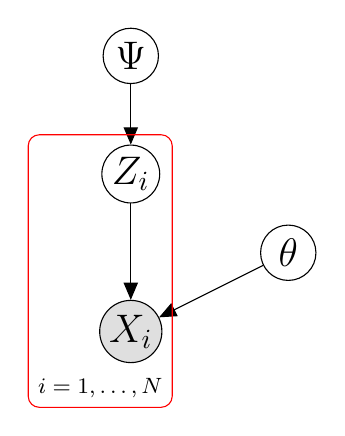
\begin{tikzpicture}
        \node[latent] (psi) at (0,1.5) {\Large $\Psi$};
        \node[latent] (z) at (0,0) {\Large $Z_i$};
        \node[obs] (x)  at (0,-2) {\Large $X_i$};
        \node[latent] (theta) at (2,-1) {\Large $\theta$};
        \path[draw,->] (z) edge (x);
        \path[draw,->] (psi) edge(z);
        \path[draw,->] (theta) edge (x);
        \plate [color=red] {part1}  {(z)(x)} {$i=1,\ldots,N$};
    \end{tikzpicture}
    \caption{Bayesian net model for variational autoencoder}
\end{figure}
In autoencoders we have some prior distribution $\Psi$. In the case of variational autoencoder we are modeling $P(X_i|Z_I)$ by neural network making it very powerfull model. Variational autoencoders
are generaiv models so they allow us to generate new data given a sample model. $p_\theta(x|z)$ is posterior modelled by neural network called  decoder. $p_\psi$ is reffered as
prior distribution.
Our model can be we are modeling:
\begin{itemize}
    \item Soft propability 
    \item Propability of 
\end{itemize}. We can also write down ELBO for VAE:
\begin{equation}
ELBO=\EX{q_\theta} [\log{p_\theta(X|Z)}]-D_{KL}(q_\phi||p_\psi)
\end{equation}. This equation is nondifferentiable in our case as numericly we want to sample from the distribution and this is non diffferentialbe. We can deal with this problem
asigning 
\begin{equation}
    Z=\mu(X)+\epsilon \sigma(X)
\end{equation}
where $\sigma$ and $\mu$ are modeld by neural networks based on $X$ and $\epsilon$ is smapled from standard normal guassian. This is differentiable and can allow us to use backpropagation to 
train encoder neural network.

\section{Sampling}

TODO

\section{Model selection}
We can divide model selection in two categories, structure learing and parameter learning. Now lets introduce new measure called mutual information
\begin{equation*}
    I(X,Y)=H(X)-H(X,I)=D_{KL}(P(X,Y)||P(X)P(Y))
\end{equation*}
If two random varibles are independent mutual information is zero! Now let's consider we have some bayesian tree $T$. We can measure weight of tree as
\begin{equation*}
    w(T)=\sum_i I(X_i,X_{pa(i)})
\end{equation*}
. We can prrove that this type of selection minimalizes divergence between orginal joint distribution and joint distribution modelled by tree. To search for such tree
we can use kruskal algorithm for maximum spanning tree with weights but weights are mutual information between varibles. To compute those values one can use maximum likelihood
estimator $f_{ij}(u,v)=P(u=i,v=j)$ to compute
\begin{equation*}
    \hat{I}(x_i,x_j)=\sum_{u,v}f_{ij}(u,v)\log{\frac{f_{ij}(u,v)}{f_i(u)f_j(v)}}
\end{equation*}. Now lets try to compute Bayes factor to compare models. We want to find $P(D|G)$ so marginalized out propability of data fiven model. We know
\begin{equation*}
    P(D|G)=\int P(D|G,\theta)P(\theta|G)\dd \theta
\end{equation*} which is hard to compute. When we assume posterior of parameter is unimodal, peeked and had a rather uninformative prior we can approximate this as
\begin{equation*}
    \log{P(D|G)}=\log{P(D|g,\hat{\theta})}+\log{\frac{\Delta \theta_{posterior}}{\Delta \theta_{prior}}}
\end{equation*} where $\hat{\theta}$ is MAP estimator. We see we have penalization for overfitting models in the form of deviation from MAP estimate which explodes if posterior
is very narrow. We can also introduce other criterions. Using Laplace expansion (assuming gaussian distribution) we can introduce
\begin{equation*}
    \log{P(D|G)}=\log{P(D|\hat{\theta},G)}-\frac{1}{2}\log{\det{H}}+\frac{\nu}{2}\log{2\pi c^2}
\end{equation*}
Where $H$ is hessian matrix of evidence defined as $E(\theta)=-\log{P(D|\theta,G)}$. Then laplace aproximation yields
\begin{equation*}
    E(\theta)\approx E(\hat{\theta})+\frac{1}{2}(\theta-\hat{\theta})^{T}\vb{H}(\theta-\hat{\theta})
\end{equation*}. When we further assume equall curvature along direction $\epsilon_i=2\pi N c^2$ where $\epsilon_i$ is eigenfunction of $H$ we get
\begin{equation*}
    \log{P(D|G)}\approx \log(D|\hat{\theta},G)-\frac{\nu}{2}\log{N}
\end{equation*}
where $\nu$ is dimension of parameter space. We can also want to use search and score aproach, we introduce graph and then by small greedy modifications we want to
find better structure. During this approach we want to score small modifications instead of score whole model. This is possible of BIC due to the fact that
BIC also decomposes as likelihood and we can introduce local score instead of global one.
\subsection{Structural EM}

\end{document}

